%\documentclass[conference]{IEEEtran}
\documentclass[12pt]{article}
\usepackage{graphicx,cite,bm,psfrag,amsmath}
\def\mmax{\mathop{\mbox{\scriptsize max}}}
\def\argmin{\mathop{\mbox{arg\,min}}}
\def\argmax{\mathop{\mbox{arg\,max}}}
\newcommand{\defequal}{\stackrel{\mathrm{def}}{=}}
\renewcommand{\vec}[1]{{\ensuremath{\boldsymbol{#1}}}}
\newcommand{\popt}{\ensuremath{P^{(K)}_{opt}}}

\pagestyle{plain}
\usepackage{amsfonts}
\usepackage{algorithm, algorithmic}
\renewcommand{\algorithmicrequire}{ \textbf{Input:}} %Use Input in the format of Algorithm
\renewcommand{\algorithmicensure}{ \textbf{Procedures:}} %UseOutput in the format of Algorithm
% correct bad hyphenation here
%\hyphenation{op-tical net-works semi-conduc-tor}
\usepackage{CJK}
\usepackage{color}
\usepackage{url}
\usepackage{geometry}
\geometry{left=0.55in, right=0.7in, top=0.75in, bottom=0.75in}

\begin{document}
\title{D.C programming with rank constrained problem}



\maketitle \thispagestyle{plain}
\pagenumbering{gobble}


% make the title area
\maketitle


\section{D.C Programming}
The D.C programming problems have been widely investigated. It has been proven that D.C programming can only converge to a  local optimal stable solution. Now we consider a digital precoder problem:
\begin{align}\label{p1}
	\text{maximize} \quad \sum_{k=1}^{K}R_k &= \sum_{k=1}^{K}\log_2\left( 1+\frac{|\bm{h}_k \bm{f}_k|^2}{\sigma_k^2 + \sum_{i\neq k}^{K}|\bm{h}_k \bm{f}_i|^2} \right)\\
	&=\sum_{k=1}^{K}\left[\log_2 \sigma_k^2 + \sum_{k=1}^{K}\left(|\bm{h}_k \bm{f}_k|^2 \right) - \log_2 \left(\sigma_k^2 + \sum_{i\neq k}^{K}|\bm{h}_k \bm{f}_i|^2\right)\right]\nonumber\\
	\text{subject to} & \quad \|\bm{V}\bm{f}_k\|_F \leq 1 ;  \nonumber\\
	& \quad R_k \geq \lambda_k,
\end{align}
where $\bm{V}$ is the analog precoder and $\bm{h}_k = \bm{w}_k^H \bm{h}_k \bm{V}$ is the effective channel.

Since $\log_2 (\cdot)$ is concave while $|\bm{h}_k \bm{f}_k|^2$ is convex, the problem \eqref{p1} can be transformed as D.C problem by defining:
\begin{align}
	\bm{F}_k = \bm{f}_k\bm{f}_k^H
\end{align} 

Then the problem \eqref{p1} can be rewritten as a standard D.C problem: 
\begin{align}\label{p2}
\text{maximize} \quad \sum_{k=1}^{K}R_k & =\sum_{k=1}^{K} \left[\log_2 \left(|\bm{h}_k \bm{F}_k\bm{h}_k^H| \right) - \log_2 \left(\sigma_k^2 + \sum_{i\neq k}^{K}|\bm{h}_k \bm{F}_i \bm{h}^H_k|\right)\right]\\
\text{subject to} & \quad \|\bm{V}\bm{f}_k\|_F \leq 1 ;  \nonumber\\
& \quad R_k \geq \lambda_k; \nonumber\\
& \quad \text{Rank}(\bm{F}_k) = 1.\nonumber
\end{align}

By ignoring the rank constraint, the digital precoder can be solved alternatively because (1) the degree freedom of variable matrix $F_k, k = 1,\cdots, K$ will be very large such that it's very hard to be solved; (2) the local optimal solution  will be sensitive to initial value as the increment of degree freedom.  We firstly give the initial value to $\bm{F}_k^{(0)}, k=1,\cdots,K$, then the digital precoder is solved iteratively:
\begin{align}\label{dc}
	\text{maximize} \quad f(\bm{F}_k) - g(\bm{F}_k): \quad\text{subject to the constraits in \eqref{p2}}  
\end{align}

The solution of problem \eqref{dc} can be calculated by iterative procedure:
\begin{align}\label{iter}
\text{maximize} \quad f(\bm{F}_k) - g(\bm{F}^{(t)}_k) - \langle\bigtriangledown g(\bm{F}^{(t)}_k), \bm{F}_k - \bm{F}^{(t)}_k\rangle: \quad\text{subject to the constraits in \eqref{p2}}  
\end{align}
This convex problem in each iterations can be easily solved by CVX toolbox.

\subsection{Convergence Analysis}
%From Taylor series expansion, we know that
%\begin{equation}
%	g(\bm{F_k}^{(t+1)}) \geq   g(\bm{F}^{(t)}_k) + <\bigtriangledown g(\bm{F}^{(t)}_k), \bm{F}_k^{(t+1)} - \bm{F}^{(t)}_k>
%\end{equation}
%Then
%\begin{equation}
%f(\bm{F_k}^{(t)}) - g(\bm{F_k}^{(t)}) \leq f(\bm{F_k}^{(t)}) - \left[ g(\bm{F}^{(t)}_k) + <\bigtriangledown g(\bm{F}^{(t)}_k), \bm{F}_k^{(t+1)} - \bm{F}^{(t)}_k>\right]
%\end{equation}

As function $g(\bm{F_k}^{(t)})$ is concave, its gradient $\bigtriangledown g(\bm{F_k}^{(t)})$ is also its super-gradient, so 
\begin{equation}
g(\bm{F_k}^{(t+1)}) \leq    g(\bm{F}^{(t)}_k) + \langle\bigtriangledown g(\bm{F}^{(t)}_k), \bm{F}^{(t+1)}_k - \bm{F}^{(t)}_k\rangle
\end{equation}
Then
\begin{equation}
f(\bm{F_k}^{(t+1)}) - g(\bm{F_k}^{(t+1)}) \geq  f(\bm{F_k}^{(t+1)}) - \left[  g(\bm{F}^{(t)}_k) + \langle\bigtriangledown g(\bm{F}^{(t)}_k), \bm{F}^{(t+1)}_k - \bm{F}^{(t)}_k\rangle\right]
\end{equation}
and from Equation (6), we know
\begin{align}
&\quad f(\bm{F}_k^{(t+1)}) - g(\bm{F}^{(t)}_k) - \langle\bigtriangledown g(\bm{F}^{(t)}_k), \bm{F}_k^{(t+1)} - \bm{F}^{(t)}_k\rangle  \nonumber\\
&\geq\quad f(\bm{F}^{(t)}_k) - g(\bm{F}^{(t)}_k) - \langle\bigtriangledown g(\bm{F}^{(t)}_k), \bm{F}_k^{(t)} - \bm{F}^{(t)}_k\rangle \nonumber \\
&=\quad f(\bm{F}^{(t)}_k) - g(\bm{F}^{(t)}_k)
\end{align}

Combining Equation (8) and (9), we have 
\begin{equation}
f(\bm{F_k}^{(t)}) - g(\bm{F_k}^{(t)}) \leq f(\bm{F_k}^{(t+1)}) - g(\bm{F_k}^{(t+1)}) 
\end{equation}

\section{The rank constrained problem}
A general rank constrained problem for SDP variable is formulated as:
\begin{align}
	\text{minimize} & \quad f(\bm{X}) \\
	\text{subject to}& \quad \bm{X} \succeq 0;\nonumber\\
	& \quad \bm{x} \in \mathcal{C}, \nonumber\\
	& \quad \text{Rank}(\bm{X})\leq r
\end{align}
where $\mathcal{C}$ is a convex set and $f(\bm{x})$ is a convex function.

This problem can be solved by an iterative method. At each step $t$,

\begin{align} \label{rank}
\min_{\bm{X}_t, e_t} & \quad f(\bm{X})  + w_t e_t \\
\text{subject to}& \quad \bm{x}_t \succeq 0;\nonumber\\
& \quad \bm{x}_t \in \mathcal{C}, \nonumber\\
&\quad e_t\bm{I}_{n-r} - \bm{U}^T_{t-1} \bm{X}_{t} \bm{U}_{t-1} \succeq \bm{0};\nonumber\\
&\quad e_t \leq e_{t-1}\nonumber
\end{align}



\section{D.C programming with rank constrained problem}

Combining the \eqref{rank} with \eqref{iter}, the $F_k$ can be solved by 
\begin{align}
\min_{\bm{X}_t, e_t} \quad -f(\bm{F}_k) + g(\bm{F}^{(t)}_k) + <\bigtriangledown g(\bm{F}^{(t)}_k), \bm{F}_k - \bm{F}^{(t)}_k> + w_t e_t
\end{align}

\begin{figure}[ht] 
	\begin{center}
		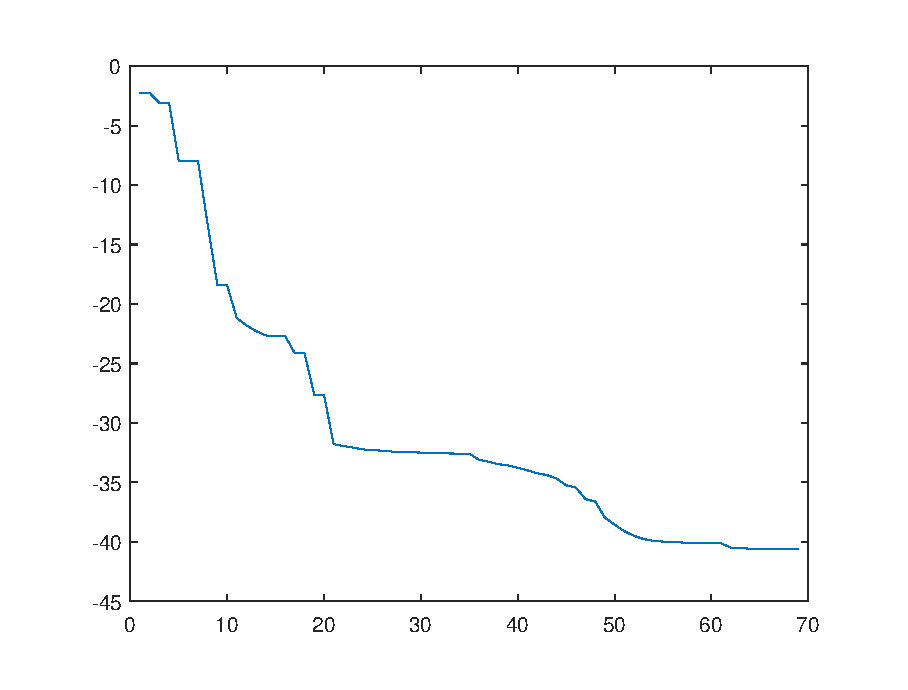
\includegraphics[width=3.6in]{t_convergence.eps}
		\caption{The convergence of proposed algorithm.}
	\end{center}
\end{figure}



\bibliographystyle{IEEEtran}
\end{document}


